\documentclass[letterpaper]{article} % DO NOT CHANGE THIS
\usepackage[submission]{aaai2027}  % DO NOT CHANGE THIS
% The serif, sans-serif, and monospaced fonts are loaded automatically by
% aaai2027.sty (newtxtext, helvet, courier). DO NOT add \usepackage{times},
% \usepackage{helvet}, \usepackage{courier}, or any other font package.
\usepackage[hyphens]{url}  % DO NOT CHANGE THIS
\usepackage{graphicx} % DO NOT CHANGE THIS
\urlstyle{rm} % DO NOT CHANGE THIS
\def\UrlFont{\rm}  % DO NOT CHANGE THIS
\usepackage{natbib}  % DO NOT CHANGE THIS AND DO NOT ADD ANY OPTIONS TO IT
\usepackage{caption} % DO NOT CHANGE THIS AND DO NOT ADD ANY OPTIONS TO IT
\frenchspacing  % DO NOT CHANGE THIS

% Recommended to typeset algorithms.
\usepackage{algorithm}
\usepackage{algorithmic}

% Recommended to typeset listings.
\usepackage{newfloat}
\usepackage{listings}
\usepackage{amsmath}
\usepackage{amssymb}
\DeclareCaptionStyle{ruled}{labelfont=normalfont,labelsep=colon,strut=off} % DO NOT CHANGE THIS
\lstset{%
    basicstyle={\footnotesize\ttfamily},
    numbers=left,numberstyle=\footnotesize,xleftmargin=2em,
    aboveskip=0pt,belowskip=0pt,
    showstringspaces=false,tabsize=2,breaklines=true}
\floatstyle{ruled}
\newfloat{listing}{tb}{lst}{}
\floatname{listing}{Listing}

% Recommended for better-looking tables.
\usepackage{booktabs}

\pdfinfo{
/TemplateVersion (2027.1)
}

\setcounter{secnumdepth}{0} % May be changed to 1 or 2 if section numbers are desired.

% Title must be in mixed case.
\title{WACBench: Evaluating Strategic Adaptation in LLM Agents through Executable Policies}

\author{Anonymous Submission}
\affiliations{}

\begin{document}

\maketitle

% Large language models are increasingly moving from assistant-style interaction toward roles that may require consequential, repeated decision making.

\begin{abstract}
Large language models (LLMs) are increasingly considered not only as assistants but as agents that may formulate and execute consequential strategies. Yet existing benchmarks often emphasize isolated actions or task completion, leaving unclear whether models can construct persistent policies and revise them under scarcity, uncertainty, delayed consequences, and strategic interdependence. We introduce WACBench, a code-mediated multi-agent benchmark built on a repeated resource-allocation game. In each meta-round, agents submit executable bidding policies that govern a complete episode and can be frozen, replayed, and inspected. Treating executable policy as the unit of evaluation removes repeated policy-to-action translation and enables comparison of stated rationale, implemented decision rules, and realized trajectories. We compare a shared self-policy-and-outcome feedback protocol with a condition that additionally reveals opponents' previous policies. Across multiple LLM backends, opponent-policy access produces more sustained gains in role-balanced survival and greater behavioral and structural convergence, while effects on mortality and individual models remain heterogeneous. WACBench provides a reproducible framework for evaluating policy construction and adaptation, showing that additional strategic information does not uniformly translate into more reliable decisions.
\end{abstract}
\noindent\textbf{Code} --- \url{https://github.com/your-anonymous-repo/code-mediated-resource-allocation}


% Uncomment the following to link to code, datasets, or an extended version.
% Keep this block between the abstract and the main body, and avoid de-anonymizing links.
% \begin{links}
%     \link{Code}{https://anonymous.4open.science/your-repository}
%     \link{Datasets}{https://anonymous.4open.science/your-dataset}
%     \link{Extended version}{https://anonymous.4open.science/your-extended-version}
% \end{links}

\section{Introduction}

Large language models (LLMs) are increasingly considered not only as
assistants that recommend actions, but also as agents that may formulate and
execute strategies on behalf of users. In settings such as resource
allocation, bidding, procurement, and organizational planning, decisions are
repeated, consequences may be delayed, and success depends on both an
uncertain environment and the behavior of other decision makers. Evaluating
isolated responses or task completion alone provides limited evidence about
whether an LLM can construct a policy that remains effective under these
conditions.

Existing agent benchmarks have substantially advanced the evaluation of
multi-step reasoning, tool use, open-ended task completion, and social
interaction~\cite{liu2023agentbench,mialon2023gaia,zhou2024sotopia,zhu2025multiagentbench}.
Game-theoretic benchmarks provide a complementary perspective by introducing
explicit objectives, strategic interdependence, and objectively measurable
outcomes. Prior work has evaluated preference formation, belief refinement,
and rational action selection in classical games~\cite{fan2024rational};
strategic reasoning across game taxonomies~\cite{duan2024gtbench,huang2025gamabench};
and planning and budget management in auctions~\cite{chen2023aucarena}.
Alympics further introduced the Water Allocation Challenge (WAC), which
combines repeated auctions, asymmetric player constraints, stochastic
scarcity, and survival dynamics~\cite{mao2025alympics}.

These environments reveal important aspects of LLM decision making, but many
evaluations still treat the action at each interaction step as the primary
unit of analysis. A model may then repeatedly translate a verbal plan into a
new action, making it difficult to determine whether success reflects a
persistent decision rule or a sequence of locally generated responses. Prior
work also shows that an LLM can overlook or modify a previously refined belief
when selecting an action~\cite{fan2024rational}. We do not assume that such
inconsistency is pervasive in current models. Instead, we argue that an
evaluation of consequential decision making should not rely on a model
faithfully reconstructing its intended policy at every step.

WACBench therefore treats an \emph{executable policy} as the unit of decision
making. An LLM first states a strategy rationale and submits a Python policy
that maps the observable game state to a bid. The simulator invokes that same
policy throughout the episode, removing repeated policy-to-action translation
from the interaction loop. Code mediation does not guarantee that the stated
rationale and implemented policy agree. Rather, it makes the implemented
decision rule persistent and ensures that its realized actions can be traced
back to submitted code. The resulting rationale, policy, and trajectory can
therefore be compared directly, while frozen policies can be replayed under
common counterfactual supply sequences. Program-based strategies have also
been used to study code-conditioned cooperation and exploitation in
open-source games~\cite{sistla2025opensourcegames}; WACBench uses their
auditability to evaluate long-horizon adaptation under resource competition.

We introduce \textbf{WACBench}, a code-mediated multi-agent benchmark built
on WAC. Five agents compete for limited daily water over a 20-day episode.
Their roles have asymmetric salary--water-requirement profiles, while all
agents share the same initial health and budget conditions. Stochastic supply,
budget depletion, health penalties, and simultaneous bidding create a
stylized stress test of policy construction under scarcity, uncertainty,
delayed consequences, and strategic interdependence. In each meta-round, an
LLM generates a policy for a complete episode and may revise that policy only
before the next meta-round.

We use this framework to study how access to opponents' decision rules changes
strategic revision. Both feedback conditions provide an agent with its own
previous policy and all agents' survival durations from the preceding
meta-round. Under \textbf{Outcome Feedback} (OF), no opponent policy or
previous-round trajectory is provided. Under \textbf{Outcome-and-Policy
Feedback} (OPF), the opponents' submitted policies are additionally revealed.
Both conditions retain identical within-episode observations of public
opponent states and past-day behavior. Their comparison therefore examines
the added value of cross-round opponent-policy access within a shared
self-revision and outcome-feedback protocol; it does not by itself establish
that a model forms an internal representation of its opponents.

Our primary evidence comes from simulator-grounded survival outcomes and
cross-meta-round adaptation. Frozen policies are replayed under common supply
sequences, and outcomes are balanced across asymmetric roles. Controlled
behavioral probes, program structure, and capability-oriented diagnostics are
used to characterize how policies change, rather than to replace objective
outcomes. An evidence-grounded failure analysis compares the stated rationale,
submitted policy, and realized trajectory, while remaining secondary to
deterministic simulator measurements.

Across the evaluated backends, opponent-policy access produces more sustained
cross-round gains in role-balanced survival, while its additional effect on
mortality and its model-level benefits remain heterogeneous. It also makes
policies more similar in both controlled bidding behavior and normalized
program structure. These findings show that policy transparency changes how
LLM agents revise executable strategies, but that additional strategic
information does not uniformly translate into more reliable decisions.

Our contributions are summarized as follows:

\begin{itemize}
    \item We introduce WACBench, a code-mediated benchmark that evaluates
    LLM agents through persistent executable policies in a repeated,
    asymmetric, and resource-constrained multi-agent environment.
    
    \item We formulate opponent-policy access as an information intervention
    by comparing a shared self-policy-and-outcome feedback protocol with the
    same protocol augmented by opponents' previous policies.
    
    \item We develop an outcome-grounded evaluation protocol that combines
    role-balanced multi-seed replay with auditable rationale--policy--trajectory
    records and controlled behavioral diagnostics.
    
    \item We show that opponent-policy access changes adaptation and is
    accompanied by behavioral and structural convergence, while its effects
    on survival reliability remain heterogeneous across model backends.
\end{itemize}
\section{Related Work}

\paragraph{LLM agent evaluation.}
General agent benchmarks emphasize multi-step task completion, tool use,
and interaction, while multi-agent benchmarks additionally study social
coordination and competition~\cite{liu2023agentbench,mialon2023gaia,zhou2024sotopia,zhu2025multiagentbench}.
WACBench instead evaluates a policy that is generated once and then acts
without further LLM intervention throughout an episode. This separates
policy construction from repeated execution and permits exact replay and
behavioral probing.

\paragraph{LLMs in games and auctions.}
Prior work uses classical games and auction environments to examine
rational choice, strategic reasoning, and budget management
~\cite{fan2024rational,duan2024gtbench,huang2025gamabench,chen2023aucarena}.
Alympics introduced WAC as a pilot environment for empirical game-theoretic
analysis and combined objective game records with human ratings of broad
strategic abilities~\cite{mao2025alympics}. We retain WAC's scarcity,
asymmetry, and survival dynamics, but shift the unit of evaluation from a
sequence of natural-language actions to persistent executable policies and
controlled cross-meta-round policy revision.

\paragraph{Program-mediated strategies.}
Program-based games make strategies reproducible and inspectable, and have
been used to study code-conditioned cooperation and exploitation
~\cite{sistla2025opensourcegames}. WACBench uses the same auditability for a
different purpose: linking a model's stated rationale, submitted code, and
realized trajectory under stochastic scarcity and strategic competition.
\section{The Repeated Water Allocation Game}
The Water Allocation Challenge (WAC), originally introduced
as a pilot environment in Alympics~\cite{mao2025alympics},
is a repeated resource-allocation game in which multiple agents compete for a limited daily water supply while managing health, budget, and long-term survival. We adopt WAC as the strategic environment underlying WACBench. Although WAC is a stylized simulation rather than a direct model of a particular real-world domain, it jointly captures several properties of real-world multi-agent decision making: scarce resources, asymmetric participants, uncertainty over future supply, and the need to balance short-term survival against long-term planning.

\subsection{Game Overview}

Each episode spans $T=20$ simulation days. At the beginning of an
episode, each agent is assigned a role specifying its daily salary $s_i$
and water requirement $w_i$. All roles begin with the same health,
budget, and no-water penalty state: $H_{i,1}=8$, $B_{i,1}=0$, and
$c_{i,1}=1$, with maximum health $H_{\max}=10$. The medium-scarcity
setting used in our experiments samples each day's integer supply as
$S_t\sim\operatorname{Unif}\{15,\ldots,25\}$. The current supply is
announced before all living agents submit simultaneous bids, but
current-day opponent bids remain hidden. The resulting four-stage daily loop
is summarized in the central panel of Figure~\ref{fig:wacbench_framework}.

\begin{table}[t]
    \centering
    \small
    \setlength{\tabcolsep}{9pt}
    \caption{Asymmetric WAC role profiles. Each role has a distinct joint
    salary--requirement profile; Alex and Cindy share a water requirement
    but differ in daily salary.}
    \label{tab:role-profiles}
    \begin{tabular}{lrr}
        \toprule
        Role & Water requirement $w_i$ & Daily salary $s_i$ \\
        \midrule
        Alex  & 13 & 70  \\
        Bob   & 9  & 90  \\
        Cindy & 13 & 150 \\
        David & 7  & 80  \\
        Eric  & 8  & 140 \\
        \bottomrule
    \end{tabular}
\end{table}

As Table~\ref{tab:role-profiles} shows, asymmetry refers to the joint
salary--requirement profiles rather than to different initial health
states. These profiles create different strategic constraints: high water
requirements make allocation more difficult when little supply remains,
while low salaries limit the bids that can be sustained over the episode.
The complete permutation evaluation rotates every model through every role
so that these structural advantages do not determine a model's aggregate
score.

Formally, let $i \in \{1,\ldots,N\}$ denote an agent and $t$ denote the
day. In addition to the fixed $s_i$ and $w_i$, each agent maintains budget
$B_{i,t}$, health $H_{i,t}$, and a no-water penalty counter $c_{i,t}$. The
counter determines the health penalty if the agent fails to obtain water
on the current day. Agents observe the announced supply and current public
states before choosing $b_{i,t}$, but do not observe other agents'
current-day bids.

\subsection{Daily Bidding, Allocation, and State Transitions}

At the start of each day, each living agent receives its
salary. Let
\begin{equation}
    \widetilde{B}_{i,t}=B_{i,t}+s_i
\end{equation}
denote the budget available for that day's auction.
The environment ranks positive feasible bids in descending order, with
ties first resolved in favor of the lower water requirement. Remaining
exact ties are resolved by a reproducible seeded tie-break. It then visits
the ranked list and allocates water to any agent whose requirement fits the
remaining supply, subtracting that requirement before considering the next
agent. Let $z_{i,t}\in\{0,1\}$ indicate whether agent $i$ receives water
on day $t$.

A winning agent pays its bid, while a non-winning agent pays
nothing:
\begin{equation}
    B_{i,t+1}
    =
    \widetilde{B}_{i,t}-z_{i,t}b_{i,t}.
\end{equation}

The no-water penalty counter is updated as
\begin{equation}
    c_{i,t+1}
    =
    \begin{cases}
        1, & z_{i,t}=1,\\
        c_{i,t}+1, & z_{i,t}=0.
    \end{cases}
\end{equation}

Health then evolves according to
\begin{equation}
    H_{i,t+1}
    =
    \begin{cases}
        \min(H_{\max},H_{i,t}+2), & z_{i,t}=1,\\
        H_{i,t}-c_{i,t}, & z_{i,t}=0.
    \end{cases}
\end{equation}
An agent is eliminated when its health reaches zero or below.

\subsection{Strategic Challenges}

WAC is strategically challenging for several reasons. First, the game is long-horizon: an agent can survive early days by spending aggressively, but this may leave insufficient budget later in the episode. Second, risk is state-dependent: low health or a high no-water counter may justify aggressive bidding, whereas the same bid may be wasteful when the agent is healthy. Third, the environment is competitive: whether a bid succeeds depends not only on supply but also on other agents' strategies. Finally, agents may be asymmetric in salary and water requirement, so a strategy that is effective for one role may fail for another.

These properties make WAC a useful testbed for evaluating whether language-model agents can produce executable policies that balance survival, budget discipline, opponent-aware adaptation, and long-term planning under uncertainty.

\section{WACBench}

WACBench evaluates strategic LLM agents through policies rather than
independently generated daily actions. Each submitted policy remains the
agent's decision rule for a complete episode, after which it can be revised,
frozen for replay, or evaluated on controlled states.

\begin{figure*}[t]
    \centering
    \includegraphics[width=\textwidth]{framework_v4.pdf}
    \caption{Overview of WACBench. The central green panel summarizes the
    four-stage daily WAC loop: announce supply, collect simultaneous bids,
    allocate water, and update agent states. Submitted rationales, executable
    policies, traces, and outcomes are stored for condition-dependent
    meta-round feedback and post-hoc evaluation. Judge annotations are
    secondary and never affect gameplay or primary outcomes.}
    \label{fig:wacbench_framework}
\end{figure*}

\subsection{Benchmark Overview}

As shown in Figure~\ref{fig:wacbench_framework}, the experiment controller
assigns backends and roles, validates submitted policies, executes each
meta-round, and stores the resulting code, traces, and outcomes. Selected
artifacts construct OF or OPF feedback for the next revision; post-hoc
diagnostics read the store without affecting gameplay.

The benchmark separates three objects that action-level evaluation can
conflate: the model's stated rationale, its implemented policy, and the
trajectory produced when that policy is executed. Simulator-grounded survival
and adaptation are the primary evidence of decision quality. Code validity,
controlled policy probes, and judge annotations characterize reliability and
failure mechanisms without replacing realized outcomes.

\subsection{Code-Mediated Agent Policies}

In each meta-round, an LLM agent receives a profile, the current game setup, and condition-dependent information about other agents. The agent produces two artifacts: a concise natural-language strategy rationale and executable Python policy code. The submitted code must define a policy of the following form:

\begin{verbatim}
def get_bid(day_context, my_status, 
opponents_status):
    ...
\end{verbatim}

The environment calls this function on every simulation day to obtain the
agent's bid. The input \texttt{day\_context} contains the current day and
announced supply; \texttt{my\_status} contains health, available budget, and
the no-water counter; and \texttt{opponents\_status} contains the public
current states and recent past-day observations of other agents. Current-day
opponent bids are never available when a policy acts.

Code mediation serves four evaluation purposes. First, it makes the policy
persistent: the simulator invokes the submitted decision rule rather than
asking the LLM to reconstruct a strategy each day. Second, it provides
policy--execution fidelity: every realized bid is attributable to a specific
program and observed state, subject to explicit validation and runtime checks.
Third, a frozen policy can be replayed under common supply sequences or probed
on controlled states. Fourth, the natural-language rationale, implemented
logic, and resulting trajectory can be audited separately. The design thus
removes repeated translation from policy to action, but deliberately retains
rationale--policy disagreement as a detectable failure mode.

\subsection{Meta-Round Adaptation and Feedback Conditions}
A meta-round is the complete policy-revision cycle. At the
beginning of meta-round $k$, each agent generates one policy
$\pi_i^{(k)}$; the simulator then executes one $T$-day episode
using that policy; finally, the resulting artifacts are stored
and selected information is used to construct feedback for
meta-round $k+1$. We use $k\in\{1,\ldots,K\}$ for meta-rounds
and reserve $t\in\{1,\ldots,T\}$ for days within an episode.

Each meta-round $k$ consists of policy generation followed by
one complete game episode. The generated policy remains fixed
during the episode and may be revised only before the next
meta-round.

For $k>1$, both feedback conditions provide the agent's own
previous policy and the vector of survival durations from the
previous meta-round. We denote this common revision memory by
\begin{equation}
    M_i^{(k)}
    =
    \left\{\pi_i^{(k-1)},
    D_1^{(k-1)},\ldots,D_N^{(k-1)}\right\}.
\end{equation}
Under \textbf{Outcome Feedback (OF)}, $F_{i,\mathrm{OF}}^{(k)}=M_i^{(k)}$.
No opponents' previous policies, bids, allocation records, daily
trajectories, or intermediate state histories are revealed.

Under \textbf{Outcome-and-Policy Feedback (OPF)}, the agent
receives the common revision memory together with the strategy
code submitted by every opponent in the previous meta-round:
\begin{equation}
    F_{i,\mathrm{OPF}}^{(k)}
    =
    M_i^{(k)}
    \cup
    \{\pi_j^{(k-1)}:j\neq i\}.
\end{equation}

The two conditions share the simulator, role assignments, own-policy memory,
outcome feedback, and within-episode observation interface. Their comparison
estimates the effect of adding opponents' policy representations within this
fixed feedback protocol. Meta-round one has no previous-round memory and
serves as a pre-feedback baseline within each condition. Because OF and OPF
use separate policy-generation runs, their MR1 policies need not be identical;
we therefore estimate policy-access effects as matched differences in changes
from the respective MR1 baselines.

\subsection{Memory, Trace Storage, and Policy Evaluation}

After each episode, WACBench stores the generated strategy code, reasoning logs, daily execution traces, and final outcomes. These records serve three purposes. First, they provide memory for later meta-rounds when the information condition allows cross-round access. Second, they support deterministic evaluation metrics such as survival days, mortality, final budget, total bid, and resource-adjusted utility. Third, they form the evidence base for judge-based diagnostic analysis.

This separation between execution and evaluation is important. The judge does not affect the game or agent behavior; it is used only after execution to interpret the stored traces. As a result, outcome metrics remain deterministic and reproducible, while the judge provides additional qualitative and structured explanations.

\subsection{Evidence-Grounded Failure Analysis}

WACBench performs post-hoc failure analysis over the stored rationale,
executable policy, and active-day trajectory. Each diagnostic item is one
agent in one experiment and meta-round whose original policy-generation
trajectory ends in death. Mechanically verifiable events---including death,
affordable threshold misses, realized payments, and prior overpayment---are
reconstructed directly from simulator records. Same-day opponent bids and
winning thresholds are marked as ex-post evidence rather than information
available to the acting policy.

The diagnostic first distinguishes whether the policy is the dominant cause,
whether policy and adverse context jointly contribute, whether no clear
policy failure is supported, or whether evidence is insufficient. A primary
mode is assigned only to the first two cases. The complete taxonomy contains
five mechanisms: fatal undercommitment, winner's-curse overpayment,
emergency-response failure, competitive-threshold miscalibration, and
allocation-rule misreasoning. Role disadvantage, unaffordable competitive
pressure, supply scarcity, and opponent-bid outliers are recorded separately
as contextual contributors and are not treated as policy failures.

Two independently queried judges (GPT-5.4 and DeepSeek V4 Flash, temperature
zero) receive the same structured evidence with the acting model's identity
hidden. Each judge contributes one-half vote to the attribution status and
primary mode. We report coverage and agreement before interpreting the
averaged distributions. We do not ask the judges for a scalar strategy score:
the diagnosis explains failed trajectories but does not replace WACScore or
mortality. Human validation on a stratified subset remains required before
final submission.

\section{Evaluation Protocol}

We organize the evaluation around three questions. First, how effective and
reliable are the submitted policies across asymmetric roles and unseen supply
sequences? Second, do policies improve across meta-rounds, and how does access
to opponents' previous policies change that adaptation? Third, what behavioral
and structural changes accompany the outcome differences? WACScore,
mortality, and cross-meta-round changes provide the primary evidence. Frozen
opponent replays, counterfactual action rollouts, risk-response probes, and
policy-convergence measures are secondary diagnostics that characterize
particular aspects of the submitted policies.

For descriptive model summaries, results are reported under Outcome Feedback
(OF), Outcome-and-Policy Feedback (OPF), and their unweighted mean,
\begin{equation}
    \operatorname{Avg}(q)
    =
    \frac{q_{\mathrm{OF}}+q_{\mathrm{OPF}}}{2},
\end{equation}
which provides a feedback-agnostic summary for metric $q$. Raw OF and OPF
levels are not interpreted as treatment effects because the two conditions
use separate policy-generation runs; policy-access effects are instead
estimated from their matched changes relative to MR1.

\subsection{Experimental Design and Uncertainty}

The heterogeneous-model evaluation enumerates all 120 assignments of
five model backends to five asymmetric roles. OF and OPF use matched
assignments. Policy generation and revision are performed under a common
base supply sequence (seed 42), ensuring that the feedback used to create
later-round policies is controlled across assignments and conditions.
After policy generation, we freeze every submitted policy and replay the
MR1--MR3 policy sets under five fixed supply seeds
$\{10,42,98,197,666\}$. These replays test whether the resulting policies
and revisions remain effective beyond the single trajectory that produced
the feedback; they do not provide the model with additional opportunities
to revise its policy.

We report 95\% confidence intervals for the primary outcome, adaptation, and
convergence estimates. For the multi-seed outcome and
adaptation analyses, the five replay outcomes are first averaged within
each experiment. Resampling is then performed over the 120 matched
experiment clusters so that the five strategically coupled agents, both
feedback conditions, and all three meta-rounds remain coupled. OF--OPF
effects are computed from matched permutation pairs. The intervals are
therefore conditional on the selected five evaluation seeds and should
not be interpreted as treating agent--seed--round observations as
independent samples.

\subsection{Outcome Metrics}

\paragraph{WACScore.}
Let $T$ be the episode horizon, $\mathcal{R}$ the set of agent roles,
$\mathcal{E}_{m,r}$ the evaluation episodes in which model $m$ occupies
role $r$, and $D_{m,r,e}\in[0,T]$ its survival duration in episode $e$.
We define
\begin{equation}
    \operatorname{WACScore}(m)
    =
    \frac{100}{|\mathcal{R}|T}
    \sum_{r\in\mathcal{R}}
    \frac{1}{|\mathcal{E}_{m,r}|}
    \sum_{e\in\mathcal{E}_{m,r}}D_{m,r,e}.
\end{equation}
WACScore is therefore 100 times the role-balanced mean fraction of the
episode survived. A score of 100 means that the model survives the full
horizon in every role, while 50 means that it survives half of the
horizon on average. Giving each role equal weight prevents frequently
sampled or intrinsically easier roles from dominating the leaderboard.

\paragraph{Mortality.}
Let $Y_{m,r,e}=1$ if the model dies during episode $e$ and $0$ otherwise.
The role-balanced mortality rate is
\begin{equation}
    \operatorname{Mortality}(m)
    =
    \frac{100}{|\mathcal{R}|}
    \sum_{r\in\mathcal{R}}
    \frac{1}{|\mathcal{E}_{m,r}|}
    \sum_{e\in\mathcal{E}_{m,r}}Y_{m,r,e}.
\end{equation}
It measures the frequency of catastrophic policy failure rather than
how early a failure occurs. Thus, WACScore captures survival effectiveness,
whereas mortality captures reliability; higher WACScore and lower
mortality are better.

\subsection{Counterfactual Planning Diagnostic}

We use paired counterfactual rollouts at fixed checkpoints, comparing
the policy bid $a_\pi$ with a discrete set $\mathcal{A}$ of budget-scaled
bids under shared future supply sequences. Counterfactual Survival
Regret (CSR) measures the expected survival days lost relative to the
best tested action:
\begin{equation}
    \mathrm{CSR}
    =
    \mathbb{E}_{s}\!\left[
        \max_{a\in\mathcal{A}}
        \mathbb{E}_{\omega}[R(s,a,\omega)]
        -
        \mathbb{E}_{\omega}[R(s,a_\pi,\omega)]
    \right],
\end{equation}
where $R(s,a,\omega)$ is remaining survival from state $s$ after action
$a$ under rollout $\omega$. Lower CSR is better; its reference is the
best tested action rather than the global continuous optimum. CSR is
conditional on the policy reaching the evaluated checkpoint.

\subsection{Risk-Response Diagnostic}

We probe generated policies offline by holding the decision context
fixed while increasing health risk, drought risk, or both. Normalized
Bid Adjustment (NBA) measures the signed change in the policy's bid
relative to available budget $B$:
\begin{equation}
    \mathrm{NBA}
    =
    \mathbb{E}\!\left[
        \frac{b_{\mathrm{risk}}-b_{\mathrm{safe}}}{B}
    \right].
\end{equation}
We average NBA over the three risk manipulations and controlled
background states. Larger values indicate a stronger upward bid
adjustment under risk; NBA is descriptive and does not by itself imply
better decision quality.

\subsection{Frozen-Opponent Revision Diagnostic}

Across meta-rounds, Frozen-Opponent Survival Gain (FOSG) measures whether
replacing only the focal MR1 policy with its MR2 revision improves
survival against unchanged MR1 opponents under common seeds:
\begin{equation}
    \mathrm{FOSG}
    =
    \mathbb{E}_{e,i,s}\!\left[
        D\!\left(\pi_i^{(2)},\pi_{-i}^{(1)};s\right)
        -D\!\left(\pi_i^{(1)},\pi_{-i}^{(1)};s\right)
    \right],
\end{equation}
where $D$ is survival in days. Positive FOSG means that the revised policy
improves survival with opponents held fixed. FOSG measures effective
revision rather than responsiveness alone; comparing it under OF and OPF
tests whether opponent-policy access improves revision, but does not
establish that the model formed an internal representation of its opponents.

\subsection{Policy Convergence}

To test whether policy transparency changes how similarly agents act, we
evaluate every submitted policy on the same grid of 144 controlled states.
The grid crosses episode stage, announced supply, available budget, health
and drought risk, and low versus high opponent-bid pressure. For policy
$\pi_i$, its behavioral signature $\mathbf{v}_i$ contains the resulting bids
after clamping them to the feasible range and normalizing by available
budget. Within each experiment, Behavioral Policy Distance (BPD) is the mean
pairwise root mean squared difference among the five signatures:
\begin{equation}
    \mathrm{BPD}
    =
    \frac{1}{\binom{N}{2}}
    \sum_{i<j}
    \sqrt{\frac{1}{Q}\sum_{q=1}^{Q}
    \left(v_{i,q}-v_{j,q}\right)^2},
\end{equation}
where $Q=144$ and lower values indicate more similar bidding behavior. The
complete permutation design balances model--role pairings across experiments.
As a structural robustness diagnostic, we additionally parse each program,
discard identifier and literal values, and compute pairwise Jaccard similarity
over AST node-type 3-grams. For both measures, the policy-access effect is the
matched difference between OPF and OF changes from the pre-feedback MR1
baseline; AST similarity is not interpreted as evidence of direct copying.

\section{Results}

\subsection{Adaptation under Policy Transparency}

We evaluate adaptation by replaying each fixed MR1--MR3 policy set under
the same five evaluation supply sequences. MR1 is the pre-feedback baseline:
neither condition has access to prior-round information. Because OF and OPF
are independent policy-generation runs, their MR1 levels need not be
identical; policy-access effects are therefore estimated as matched
differences in changes from MR1. The transition from MR1 to MR2 measures the
first revision, while MR2 to MR3 distinguishes continued improvement from
saturation or regression.

\begin{figure}[t]
    \centering
    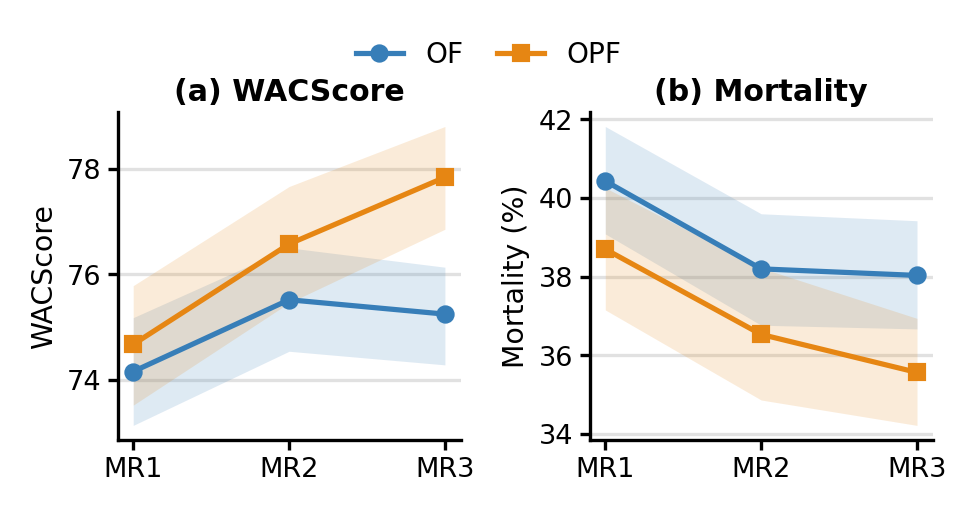
\includegraphics[width=\linewidth]{adaptation_trajectories.png}
    \caption{Cross-meta-round adaptation under Outcome Feedback (OF) and
    Outcome-and-Policy Feedback (OPF). Policies from each meta-round are
    replayed under five fixed supply sequences. Points are role-balanced
    estimates after averaging seeds within experiments; shaded regions are
    95\% matched experiment-cluster bootstrap intervals.}
    \label{fig:adaptation-trajectories}
\end{figure}

Figure~\ref{fig:adaptation-trajectories} shows improvement after the first
revision under both conditions, but their later dynamics diverge. OF largely
plateaus after MR2, whereas OPF continues to improve through MR3. Across the
full revision horizon, the OPF increase in WACScore exceeds the OF increase
by 2.08 points (95\% CI $[0.46,3.77]$). Mortality declines under both
conditions, but the difference between their reductions remains uncertain.
Policy transparency therefore more clearly improves survival duration than
the probability of avoiding every catastrophic failure.

The aggregate effect is highly heterogeneous. GPT-5.4 Nano has the largest
baseline-adjusted MR1-to-MR3 effect: $+11.53$ WACScore points (95\% CI
$[4.28,18.80]$) and $-11.83$ mortality points ($[-21.32,-2.27]$). The other
model-specific intervals include zero. This pattern does not support a
simple strong-model advantage-amplification account; instead, the largest
measured benefit accrues to the backend that performs worst under OF. Full
model-level estimates are reported in the appendix.

\subsection{Overall Policy Effectiveness and Reliability}

Table~\ref{tab:outcome-performance} provides descriptive context for the
adaptation results by reporting the two simulator-grounded outcome metrics
for revised policies in MR2--MR3. Gemini 3.5 Flash achieves the highest
WACScore under both feedback conditions and maintains low mortality. Claude
Sonnet 5 and GPT-5.4 form a second performance tier, whereas DeepSeek V4
Flash and GPT-5.4 Nano have weaker feedback-averaged outcomes. These raw
condition levels combine distinct MR1 realizations and should not be read as
policy-access effects; the matched changes reported above provide the
appropriate comparison. Corresponding matched-cluster intervals are reported
in the appendix.

\begin{table}[t]
    \centering
    \small
    \setlength{\tabcolsep}{5pt}
    \caption{Simulator-grounded performance of revised policies, averaged
    over MR2--MR3 and five fixed supply sequences. Estimates are
    role-balanced. Avg. is the unweighted mean across OF and OPF; raw
    condition levels are descriptive rather than baseline-adjusted effects.}
    \label{tab:outcome-performance}
    \begin{tabular}{lrrr rrr}
        \toprule
        & \multicolumn{3}{c}{WACScore $\uparrow$}
        & \multicolumn{3}{c}{Mortality (\%) $\downarrow$} \\
        \cmidrule(lr){2-4}\cmidrule(lr){5-7}
        Model & OF & OPF & Avg. & OF & OPF & Avg. \\
        \midrule
        Gemini 3.5 Flash  & \textbf{86.47} & \textbf{87.05} & \textbf{86.76} & 25.75 & \textbf{25.08} & \textbf{25.42} \\
        Claude Sonnet 5   & 86.17 & 84.05 & 85.11 & \textbf{25.00} & 28.67 & 26.83 \\
        GPT-5.4           & 84.27 & 81.72 & 83.00 & 27.58 & 31.08 & 29.33 \\
        DeepSeek V4 Flash & 69.04 & 67.84 & 68.44 & 45.83 & 46.58 & 46.21 \\
        GPT-5.4 Nano      & 50.95 & 65.35 & 58.15 & 66.42 & 48.83 & 57.62 \\
        \bottomrule
    \end{tabular}
\end{table}

\subsection{Policy Convergence}

\begin{figure}[t]
    \centering
    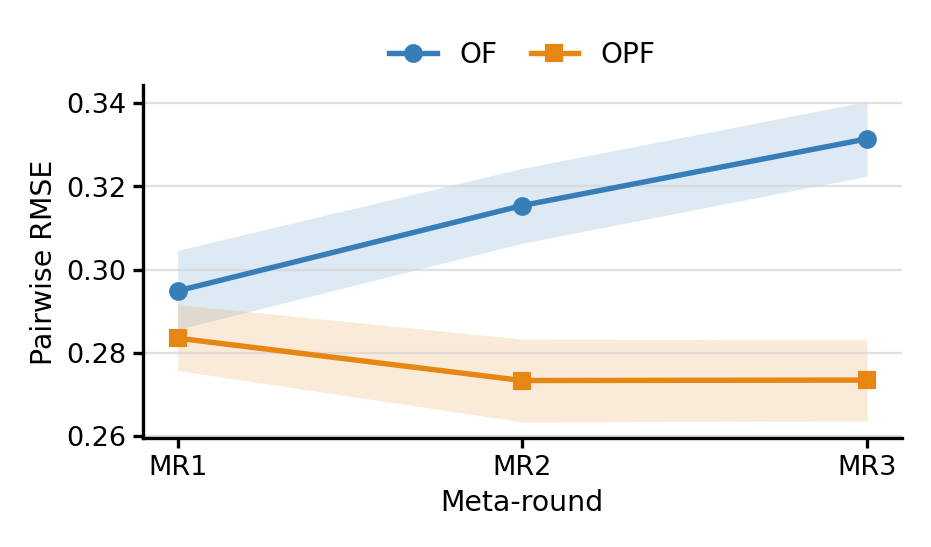
\includegraphics[width=0.90\linewidth]{policy_convergence.png}
    \caption{Behavioral convergence across meta-rounds. Distance is the
    within-experiment mean pairwise RMSE between normalized bids on 144
    controlled states; lower values indicate more similar behavior. Shaded
    regions are 95\% matched experiment-cluster bootstrap intervals.}
    \label{fig:policy-convergence}
\end{figure}

Figure~\ref{fig:policy-convergence} shows that the two feedback conditions
produce qualitatively different policy dynamics. Under OF, behavioral
distance increases across revisions; under OPF, it decreases after the first
policy exposure and then remains stable. From MR1 to MR3, the OPF-minus-OF
change in behavioral distance is $-0.0467$ (95\% CI
$[-0.0613,-0.0325]$). The structural diagnostic agrees: the corresponding
difference in AST similarity is $+0.0928$ ($[0.0826,0.1029]$). All 518,400
policy--probe evaluations execute successfully. The structural trajectory is
reported in the appendix.

Cross-model outcome dispersion moves in the same descriptive direction:
from MR1 to MR3, WACScore and mortality dispersion rise under OF but decline
under OPF. The baseline-adjusted dispersion intervals, however, approach or
include zero, so we treat performance compression as supporting descriptive
evidence rather than a separate confirmatory result. Together, the probe and
outcome analyses show that access to opponents' decision rules changes the
policy-revision process in a shared direction. They do not distinguish
strategic learning from imitation, establish that agents copy a particular
opponent, or imply that greater similarity is intrinsically optimal.

\subsection{Secondary Policy Diagnostics}

Table~\ref{tab:capability-diagnostics} complements final outcomes with
three task-motivated diagnostics: CSR for checkpoint-level planning, NBA for
risk-conditioned bid adjustment, and FOSG for revision against frozen
opponents. These measures describe particular aspects of policy behavior;
they are neither an exhaustive definition of strategic competence nor a
substitute for simulator-grounded outcomes.

\begin{table}[t]
    \centering
    \small
    \setlength{\tabcolsep}{3.2pt}
    \caption{Secondary policy diagnostics under OF and OPF. CSR and
    FOSG are measured in survival days; NBA is a percentage of available
    budget and has no monotonic better direction. FOSG uses valid paired
    MR1-to-MR2 replays.}
    \label{tab:capability-diagnostics}
    \begin{tabular}{llrrr}
        \toprule
        Model & Feedback & CSR $\downarrow$ & NBA (\%) & FOSG $\uparrow$ \\
        \midrule
        Gemini 3.5 Flash
            & OF  & 0.091 & 29.0 & 0.471 \\
            & OPF & 0.080 & 28.1 & 0.259 \\
            & Avg. & 0.086 & 28.6 & 0.365 \\
        \addlinespace
        Claude Sonnet 5
            & OF  & \textbf{0.037} & 16.3 & \textbf{1.012} \\
            & OPF & \textbf{0.030} & 18.5 & 0.835 \\
            & Avg. & \textbf{0.033} & 17.4 & \textbf{0.923} \\
        \addlinespace
        GPT-5.4
            & OF  & 0.054 & 22.4 & 0.596 \\
            & OPF & 0.096 & 23.1 & \textbf{0.927} \\
            & Avg. & 0.075 & 22.7 & 0.762 \\
        \addlinespace
        DeepSeek V4 Flash
            & OF  & 0.439 & 13.7 & 0.068 \\
            & OPF & 0.320 & 15.1 & 0.590 \\
            & Avg. & 0.379 & 14.4 & 0.329 \\
        \addlinespace
        GPT-5.4 Nano
            & OF  & 0.608 & 7.7 & $-0.284$ \\
            & OPF & 0.394 & 11.1 & 0.131 \\
            & Avg. & 0.501 & 9.4 & $-0.076$ \\
        \bottomrule
    \end{tabular}
\end{table}

In the counterfactual planning diagnostic, Claude achieves the lowest average CSR. DeepSeek
and GPT-5.4 Nano show substantially higher survival regret, although OPF
reduces CSR for both. GPT-5.4 instead has higher CSR under OPF, indicating
that the effect of policy transparency on checkpoint-level action quality
is model dependent.

In the risk-response diagnostic, Gemini makes the largest normalized bid adjustments under risk, while
GPT-5.4 Nano makes the smallest. OPF modestly increases NBA for four
models but slightly decreases it for Gemini. Because NBA measures the
magnitude and direction of a policy response rather than its realized
value, these differences should not be interpreted as a capability
ranking by themselves.

Claude has the largest average FOSG, while GPT-5.4 has the largest FOSG
under OPF. GPT-5.4 Nano changes from a negative FOSG under OF to a small
positive value under OPF, and DeepSeek also improves. These heterogeneous
effects show why effective revision must be distinguished from policy
change alone; WACScore and mortality remain the primary measures of
decision quality.

\subsection{Failure Mechanisms in Unsuccessful Policies}

Table~\ref{tab:outcome-performance} already reports how frequently models
die under multi-seed replay. We therefore use the judge only to ask how the
original failed trajectories differ, rather than repeating mortality in a
second figure. Among 3,600 valid agent-rounds in the policy-generation
trajectories, 1,444 end in death; all receive valid outputs from both judges.
These cases come from the common generation supply sequence and should not be
confused with the five-seed replay population in
Table~\ref{tab:outcome-performance}.

The attribution stage does not force every death into a policy category.
Averaging the two judges' votes, 67.9\% of deaths are attributed primarily to
the policy, 22.4\% to a combination of policy and adverse context, 9.5\% have
no clear policy failure, and 0.2\% have insufficient evidence. Thus, 90.2\%
of deaths support at least partial policy attribution;
Figure~\ref{fig:failure-modes} shows the primary-mode composition of this
attributable subset.

\begin{figure}[t]
    \centering
    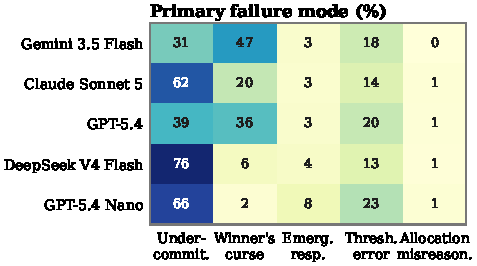
\includegraphics[width=\linewidth]{failure_analysis_figures/primary_failure_heatmap.pdf}
    \caption{Primary failure modes among policy-attributable deaths in the
    original policy-generation trajectories. Each blinded judge contributes
    one-half vote, and every row is normalized over deaths attributed wholly
    or partly to the submitted policy. The complete five-mode taxonomy is
    retained, including rare allocation-rule misreasoning. Values are rounded
    percentages and represent diagnostic annotations rather than
    simulator-defined causal ground truth.}
    \label{fig:failure-modes}
\end{figure}

Figure~\ref{fig:failure-modes} reveals different failure signatures despite
the shared game interface. Fatal undercommitment accounts for 75.7\% of
DeepSeek V4 Flash's attributable deaths and 66.0\% of GPT-5.4 Nano's. Gemini
3.5 Flash instead has a winner's-curse-heavy profile (47.3\%), consistent with
policies that secure costly earlier wins at the expense of later budget. This
operationalizes the overpayment mechanism observed in the original WAC study
~\cite{mao2025alympics}. GPT-5.4 is divided between undercommitment (39.2\%)
and winner's-curse overpayment (36.4\%), while competitive-threshold
miscalibration remains a secondary but recurrent diagnosis across models.
Allocation-rule misreasoning is below 1\% overall; retaining it shows that
explicit misunderstanding of the allocation mechanism is rare relative to
bid calibration and intertemporal budget errors.

Attribution-status agreement is 81.2\% ($\kappa=0.610$), whereas exact
primary-mode agreement is 61.6\% ($\kappa=0.436$). We therefore interpret the
heatmap as an averaged diagnostic distribution, not a definitive causal
labeling of individual deaths. Contextual contributors, judge-specific
counts, death-conditioned rationale--policy and policy--trajectory mismatch,
and human-validation results are reserved for the appendix.

\section{Limitations}

WACBench studies one stylized resource-allocation game, and policy
revision is generated from feedback under a single base supply
trajectory. Although replaying the fixed policies under five evaluation
seeds tests robustness to additional scarcity realizations, the reported
uncertainty remains conditional on this selected seed set and does not
capture the full distribution of possible environments. Code mediation
also evaluates a model's ability to formulate an executable policy under
a restricted interface, which is narrower than unconstrained interactive
agency and does not guarantee agreement between a model's verbal rationale
and its submitted program. Moreover, OF and OPF branch from separately
generated MR1 policies rather than an identical shared policy set. Matched
differences in changes adjust for their observed MR1 levels, but cannot remove
all variation due to independent policy generation. Performance is also
conditional on the selected backend pool; adding heuristic reference policies
or other opponent populations would provide a stronger absolute calibration
of benchmark difficulty. The convergence probes cover a fixed,
task-motivated state grid;
behavior outside this grid may differ, and similarity does not by itself
imply strategic optimality or direct copying from a particular opponent.
Finally, LLM-judge annotations remain interpretive even when grounded in
reconstructed evidence. We mitigate this limitation through two independent
judges, model-name blinding, explicit non-policy attribution options, and by
keeping all judge outputs secondary to deterministic simulator outcomes.
Exact primary-mode agreement is moderate, and the planned stratified human
validation is necessary before treating the taxonomy as reliable beyond the
reported diagnostic use.

\section{Conclusion}

We introduced WACBench, a code-mediated benchmark for evaluating strategic
adaptation in a repeated, asymmetric resource competition environment.
Treating executable policies as the unit of decision making makes the
implemented decision rule persistent, permits exact replay, and exposes the
links among a model's rationale, policy, actions, and realized trajectory.
Across five backends, opponent-policy feedback has heterogeneous effects, but
multi-seed replays reveal a clear aggregate revision pattern: OF largely
plateaus after its first revision, whereas OPF sustains WACScore gains through
the final meta-round. Its additional effect on mortality is less certain.
Controlled probes further show convergence in bidding behavior and program
structure under OPF, with the largest performance benefit accruing to
GPT-5.4 Nano rather than the strongest backend. These results show that
access to opponents' executable strategies changes policy revision, but does
not uniformly produce more reliable decisions. Failure diagnosis further
separates undercommitment-heavy deaths in DeepSeek V4 Flash and GPT-5.4 Nano
from the winner's-curse-heavy profile of Gemini 3.5 Flash. More broadly, the
results motivate
evaluating strategic agents through persistent policies, common-environment
replays, objective outcomes, and auditable failure mechanisms.

% Uncomment and replace with your bibliography file when ready.
\bibliography{aaai2027}

\end{document}